\documentclass{beamer}
\usetheme{Warsaw}  %% Themenwahl

\title{WearLoc}
\author{L. Gemein, D. Speck, A. Biedekapp, R. Gelhausen, J. Nist}
\date{\today}

\begin{document}
\maketitle

\begin{frame} %%Eine Folie
  \frametitle{WearLoc}%%Folientitel
  \begin{center}Simultaneous Localization and Mapping (SLAM)
  \end{center}
  \begin{figure}
  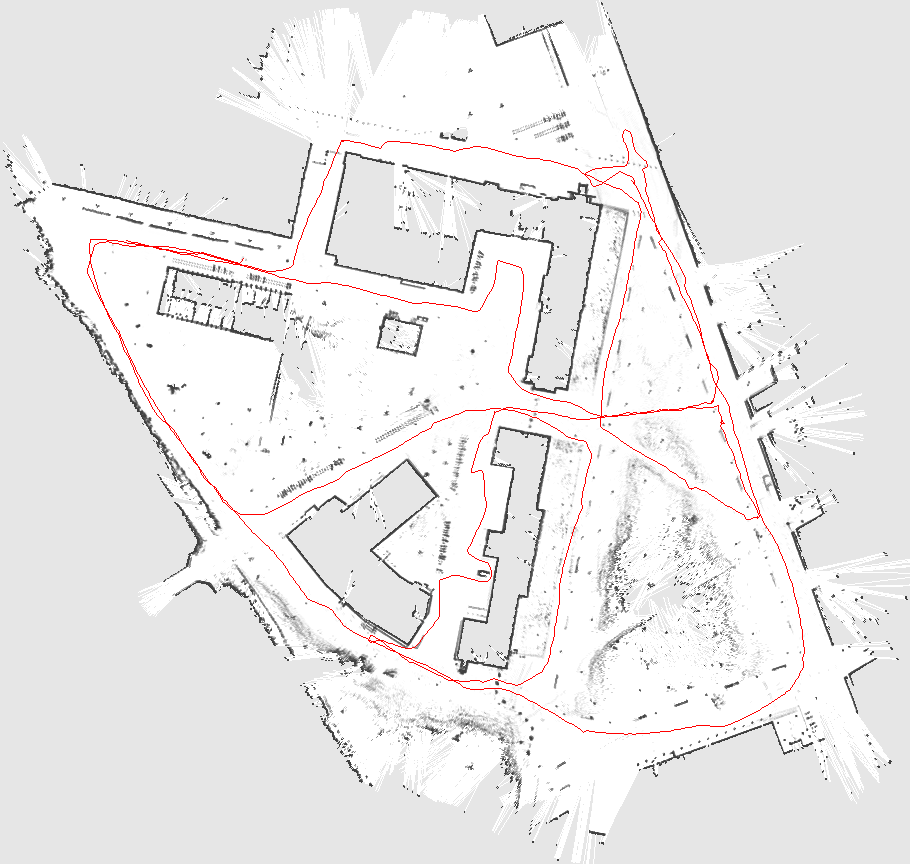
\includegraphics[width=0.5\textwidth]{slam.png} 
  \caption{SLAM: \url{http://wiki.ros.org/slam_gmapping/Tutorials/MappingFromLoggedData}}
  \end{figure}
\end{frame}

\begin{frame}
\frametitle{Setup}
\begin{minipage}[l]{0.5\textwidth}
\begin{itemize}
\item Intel Edision
\item ROS SLAM
\item Laserscanner
\item Position sensors
\end{itemize}
\end{minipage}
\begin{minipage}[r]{0.4\textwidth}
  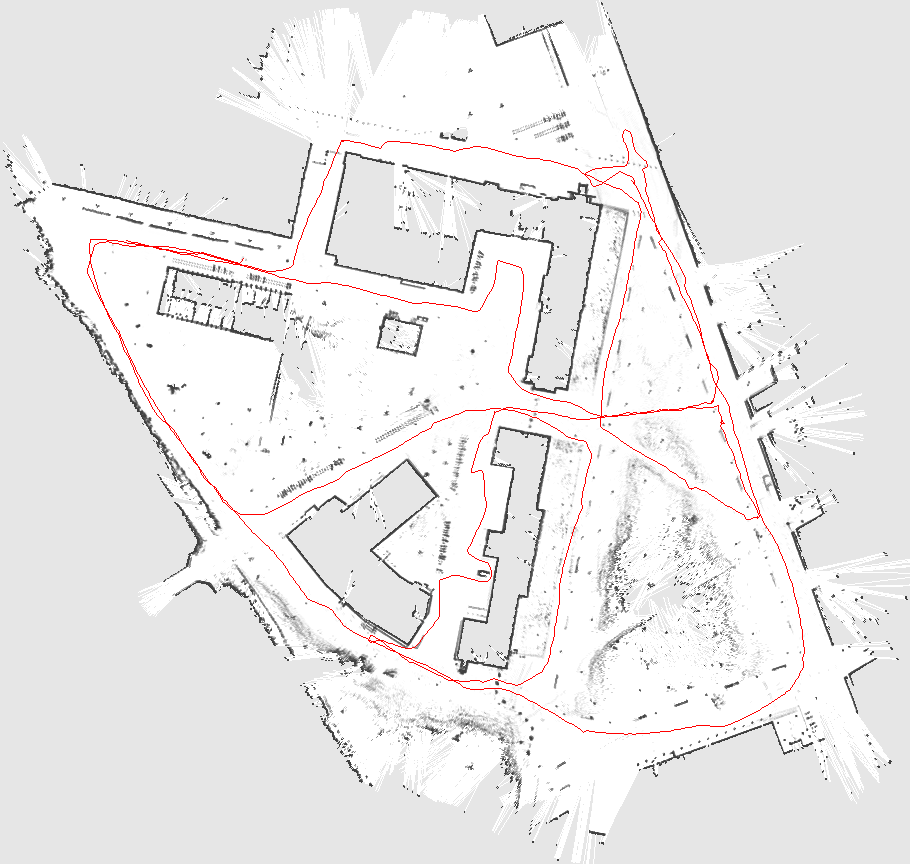
\includegraphics[width=1\textwidth]{slam.png} 
\end{minipage}
\end{frame}

\begin{frame}
\frametitle{Workplan}
\begin{itemize}
\item \textbf{04.05.2016: Group presentations}
\item 2 weeks: installing ROS + connecting Sensor
\item 2 weeks: prepearing data (calibrations) + writing interface
\item 1 week: time buffer 
\item \textbf{08.06.2016: Mid-Term Presentations} \\
$\Rightarrow$ all necessary data available/accessible in ROS
\item 2 weeks: first SLAM + calibrations
\item 2 weeks: refinements + design
\item 2 weeks: time buffer
\item \textbf{20.07.2016: Final Presentations} \\
$\Rightarrow$ working WearLoc version + (live presentation) 
\end{itemize}
\end{frame}


\begin{frame}
\frametitle{Division of Task}
\begin{itemize}
\item Organisation: Jennifer
\item Hardware: Lukas and Jennifer
\item Data management: Andr\'e, Rick and David
\item ROS: David and Lukas
\item Presentation: David, Lukas and Jennifer
\item Poster: Andr\'e
\item Paper: Rick
\end{itemize}
\end{frame}

\begin{frame}
\frametitle{Backup strategies}
\begin{itemize}
\item Plan A: Computing on chip Intel Edison
\item Plan B: Transmission via wifi to more powerful devices 
\item Plan C: Collecting data and 'post-computation' on computer
\end{itemize}
\end{frame}

\end{document}